\documentclass{report}

\usepackage[utf8]{inputenc}
\usepackage[T1]{fontenc}
\usepackage{mathtools}
\usepackage[thinc]{esdiff}


\begin{document}
	
	\chapter{Probability Theory}
	
	\section{}
	(a) S = \{HHHH, HHHT, HHTH, HHTT, HTHH, HTHT, HTTH, HTTT, THHH, THHT, THTH, THTT, TTHH, TTHT, TTTH, TTTT\} \newline
	(b) S = A countable set \newline
	(c) S = A countable set \newline
	(d) S = \(5g, 7g\) \newline
	(e) S = [0, 100\%]
	
	\section{}
	(a) We know A{\textbackslash}B = A$\cap$B\textsuperscript{C}. Let $\phi$ be the null set. So it can be written as \newline
	
	A $\cap$ B\textsuperscript{C} = $\phi$ $\cup$ (A $\cap$ B\textsuperscript{C})

	A $\cap$ B\textsuperscript{C} = (A $\cap$ A\textsuperscript{C}) $\cup$ (A $\cap$ B\textsuperscript{C})
	
	From Distribution Law
	
	(A $\cap$ A\textsuperscript{C}) $\cup$ (A $\cap$ B\textsuperscript{C}) = A $\cap$ (A\textsuperscript{C} $\cup$ B\textsuperscript{C}) = A $\cap$ (A $\cap$ B)\textsuperscript{C} = A{\textbackslash}(A$\cap$B) 
	
	$\newline$
	
	(b) Let U be the universal set containing both A and B. \linebreak
	$\newline$
	B = B $\cap$ U $\Rightarrow$ B = B $\cap$ (A $\cup$ A$\textsuperscript{C}$) $\Rightarrow$ (B $\cap$ A) $\cup$ (B $\cap$ B$\textsuperscript{C}$)
	
	$\newline$
	
	(c) By Definition
	
	$\newline$
	
	(d) A $\cup$ B = (A $\cup$ B) $\cap$ U $\Rightarrow$ (A $\cup$ B) $\cap$ (A $\cup$ A$\textsuperscript{C}$) $\Rightarrow$ A $\cup$ (B $\cap$ A$\textsuperscript{C}$)
	$\newline$
	
	\section{}
	(a) To Prove {A $\cup$ B} = {B $\cup$ A}
	
	To prove that two sets are equal, it must be demonstrated that each set contains the other. Formally
	
	A $\cup$ B = \{x $\epsilon$ S: x $\epsilon$ A or x $\epsilon$ B\} $\Rightarrow$ \{x $\epsilon$ S: x $\epsilon$ B or x $\epsilon$ A\}
	= B $\cup$ A
	
	Same logic goes for A $\cap$ B = B $\cap$ A
	$\newline$
	$\newline$
	(b) To prove A $\cup$ (B $\cup$ C) = (A $\cup$ B) $\cup$ C
	
	We first show A $\cup$ (B $\cup$ C) $\subset$ (A $\cup$ B) $\cup$ C
	$\newline$
	Let x $\epsilon$ (A $\cup$ (B $\cup$ C)) $\Rightarrow$ x $\epsilon$ A or x $\epsilon$ (B $\cup$ C) $\Rightarrow$ x $\epsilon$ B or x $\epsilon$ C.
	So it could mean that x $\epsilon$ (A $\cup$ B) or x $\epsilon$ C $\Rightarrow$ x $\epsilon$ ((A $\cup$ B) $\cup$ C) So our subset hypothesis is correct. Now $\newline$
	
	Let us show (A $\cup$ B) $\cup$ C $\subset$ A $\cup$ (B $\cup$ C)
	$\newline$
	Let x $\epsilon$ (A $\cup$ B) $\cup$ C $\Rightarrow$ x $\epsilon$ C or x $\epsilon$ (A $\cup$ B) $\Rightarrow$ x $\epsilon$ A or x $\epsilon$ B.
	So it could mean that x $\epsilon$ A  or x $\epsilon$  (B $\cup$ C) $\Rightarrow$ x $\epsilon$ (A $\cup$ (B $\cup$ C)) So our subset hypothesis is correct.
	
	Same goes with other parts. 
	
	$\newline$
	(c) Same as (b)
	
	\section{}
	(a) P(A $\cup$ B) = P(A) + P(B) - P(A $\cap$ B)
	$\newline$
	(b) P((A $\cup$ B) {\textbackslash} (A $\cap$ B)) = P(A) + P(B) - 2 * P(A $\cap$ B)
	$\newline$
	(c) (d)not cleat to me
	
	\section{}
	(a) A $\cap$ B $\cap$ C = \{a U.S birth results in identical twin females\}
	$\newline$
	(b) P(identical twins (one-egg)) = 1/3 $\newline$  P(fraternal twins (one-egg)) = 2/3
	
	P(a U.S birth results in twins) = 1/90
	
	So birth of identical twins with females = 1/2 * 1/3 * 1/90 = 1/540
	
	\section{}
	Let c1 = coin 1
	Let c2 = coin 2
	$\newline$
	P(head$\textsubscript{c1}$) = w
	$\newline$
	P(head$\textsubscript{c2}$) = v
	$\newline$
	p$\textsubscript{0}$ = (1-u) * (1-w)
	$\newline$
	p$\textsubscript{1}$ = (1-u) * w + u * (1-w)
	$\newline$
	p$\textsubscript{2}$ = uw
	$\newline$
	(1-u) * (1-w) = (1-u) * w + u * (1-w)
	$\newline$
	u * w = (1-u) * (1-w)
	$\newline$
	On solving u,w = (1, 1/2) or (1/2, 1)
	$\newline$
	
	\section{}
	(a) \newline
	P(Area after hitting the i$\textsuperscript{th}$ ring) = $\pi$((6-i)$\textsuperscript{2}$ - (5-i)$\textsuperscript{2}$)r$\textsuperscript{2}$ / (5{\textsuperscript{2}} * A)
	$\newline$
	
	(b) \newline
	P(board is hit) = $\pi$r${\textsuperscript{2}}$ / A
	$\newline$
	P(scoring i points $\vert$ board is hit) = P(scoring i points) / P(board is hit)
	$\newline$
	= ((6-i)$\textsuperscript{2}$ - (5-i)$\textsuperscript{2}$) / 5$\textsuperscript{2}$
	
	\section{}
	(a) 	P(scoring i points) = ($\pi$(6-i)$\textsuperscript{2}$ - $\pi$(5-i)$\textsuperscript{2}$)r$\textsuperscript{2}$ / (25)
	$\newline$
	(b) dP/di = -2 (As points increase scoring them decrease)
	$\newline$
	(c) According to Kolmogorov Axioms
	$\newline$
	i) On simplifying P it results in P = 11 - 2i / 25. Clearly for i=\{1, 2, 3, 4, 5\} P(i) $>$ 0 satisfying 1{\textsuperscript{st}} axiom
	$\newline$
	ii) Let S be sample space. Sample is complete dart board, So if we score in the dartboard we get 1.
	$\newline$
	iii) All the region have a pairwise disjoint nature (i=1 with i=3 for example) They do not share a common boundary. Hence P(A$\textsubscript{i}$ $\cap$ A$\textsubscript{j}$) = $\phi$ where A$\textsubscript{i}$ $\subset$ S. So if P(A$\textsubscript{i}$ $\cup$ A$\textsubscript{j}$ $\cup$ A$\textsubscript{k}$) = P(A$\textsubscript{i}$) + P(A$\textsubscript{j}$ $\cup$ A$\textsubscript{k}$) - P(A$\textsubscript{i}$ $\cap$ (A$\textsubscript{j}$ $\cup$ A$\textsubscript{k}$)) =  P(A$\textsubscript{i}$) + P(A$\textsubscript{j}$) + P(A$\textsubscript{k}$) - P((A$\textsubscript{i}$ $\cap$ A$\textsubscript{j}$) $\cup$ (A$\textsubscript{i}$ $\cap$ A$\textsubscript{k}$)) = P(A$\textsubscript{i}$) + P(A$\textsubscript{j}$) + P(A$\textsubscript{k}$)
	$\newline$
	If we generalize P($\bigcup\limits_{i=1}^{\infty} A_{i}$) = $\sum\limits_{i=1}^{\infty} P(A_{i})$
	
	\section{}
	(a) ({$\cup$}{$\textsubscript{$\alpha$}$}$\textit{A}${\textsubscript{$\alpha$}})$\textsuperscript{c}$ = ($\textit{A{\textsubscript{1}}}$ $\cup$ $\textit{A{\textsubscript{2}}}$ $\cup$ $\textit{A{\textsubscript{3}}}$ ...)$\textsuperscript{c}$ = $\textit{A}^{c}_{1}$ $\cap$ ($\textit{A}_{2}$ $\cup$ $\textit{A}_{3}$ $\cup$ $\textit{A}_{4}$ ... )$\textsuperscript{c}$ = $\textit{A}^{c}_{1}$ $\cap$ $\textit{A}^{c}_{2}$ $\cap$ ($\textit{A}_{3}$ $\cup$ $\textit{A}_{4}$ $\cup$ $\textit{A}_{5}$ ... )$\textsuperscript{c}$ = ... = $\textit{A}^{c}_{1}$ $\cap$ $\textit{A}^{c}_{2}$ $\cap$ $\textit{A}^{c}_{3}$ $\cap$ $\textit{A}^{c}_{4}$ ... = $\cup$$\textsubscript{$\alpha$}$${\textit{A}}^{c}_{\alpha}$
	
	(b) Kindly look above and go through the same path!
	
	\section{}
	Kindly Refer section 1.9 the same approach.
	
	\section{}
	(a) Given $\beta$ = \{{$\phi$}, S\}
	
	Criteria (i) is satisfied for sigma algebra.
	
	Since S is also available S{\textsuperscript{c}} = {$\phi$} (ii) Criteria is satisfied.
	
	{$\phi$} $\phi$ S = S. S {$\subset$} {$\beta$}. Hence (iii) criteria is also satisfied.
	{$\newline$}
	(b) {$\beta$} = {all subsets of S} So {$\phi$} {$\subset$} S. So, criteria (i) is satisfied. Let A {$\subset$} S {$\Rightarrow$} A{\textsuperscript{c}} {$\subset$} S. So (ii) is justified. Let A{\textsubscript{c1}}, A{\textsubscript{c2}}, A{\textsubscript{c3}} ... are subset of S. So A{\textsubscript{i}} $\cup$ A{\textsubscript{j}} $\subset$ S also A{\textsubscript{i}} $\cup$ A{\textsubscript{j}} $\in$ {\textit{$\beta$}}. So (A{\textsubscript{i}} $\cup$ A{\textsubscript{j}}){\textsuperscript{c}} {$\subset$} S. (Because we have only chosen from sample space). (A{\textsubscript{i}} $\cup$ A{\textsubscript{j}}){\textsuperscript{c}} {$\in$} {\textit{$\beta$}}. Hence Criteria (iii) for sigma algebra is justified.
	{\newline}
	(c) Let {\textit{$\beta$}}$\textsubscript{1}$ and {\textit{$\beta$}}$\textsubscript{2}$ are two sigma algebra. 
	
	{$\phi$} {$\in$} {\textit{$\beta${\textsubscript{1}}}} and {$\phi$} {$\in$} {\textit{$\beta${\textsubscript{2}}}} {$\Rightarrow$} {$\phi$} {$\in$} {\textit{$\beta${\textsubscript{1}} $\cap$  $\beta${\textsubscript{2}}}}. Hence 1{\textsuperscript{st}} criteria is satisfied.
	Let A {$\in$} {$\beta${\textsubscript{1}},{$\beta${\textsubscript{2}} So A {$\in$} {\textit{$\beta${\textsubscript{1}} $\cap$  $\beta${\textsubscript{2}}}} {$\Rightarrow$} A{\textsuperscript{c}}} {$\in$} {\textit{$\beta${\textsubscript{1}} $\cap$  $\beta${\textsubscript{2}}}} (Because A{\textsuperscript{c}} would be in both of {\textit{$\beta${\textsubscript{1}}}} and {\textit{$\beta${\textsubscript{2}}}}, referring to definition of Sigma Algebra). Hence Criteria (ii) also satisfied.
	{$\bigcup\limits_{i=1}^{\infty} A_{i}$ = S} {$\in$} {\textit{$\beta${\textsubscript{1}}}} and {$\bigcup\limits_{j=1}^{\infty} A_{j}$ = S} {$\in$} {\textit{$\beta${\textsubscript{1}}}}. Upon intersection {S} {$\in$} {\textit{$\beta${\textsubscript{1}} $\cap$  $\beta${\textsubscript{2}}}}. Hence (iii) is implemented.
	
	\section{}
	(a) P({$\bigcup\limits_{j=1}^{\infty} A_{j}$}) = P(A{\textsubscript{1}} {$\cup$} A{\textsubscript{2}} {$\cup$} A{\textsubscript{3}} ... ) = P(A{\textsubscript{1}} {$\cup$} (A{\textsubscript{2}} {$\cup$} A{\textsubscript{3}} ... )) = P(A{\textsubscript{1}}) + P(A{\textsubscript{2}} {$\cup$} A{\textsubscript{3}} {$\cup$} A{\textsubscript{4} ... }) as A{\textsubscript{1}}, A{\textsubscript{2}}, A{\textsubscript{3}} ... are pairwise disjoint so the intersection of A{\textsubscript{1}} with the rest of the unions of elements would be {$\phi$} Let B = {A{\textsubscript{2}} {$\cup$} A{\textsubscript{3}} {$\cup$} A{\textsubscript{4}} ... }. By definition of sigma algebra Axiom (iii), B {$\in$} {\textit{B}}. So B {$\in$}{\textit{B}}. On Simplification P(A {$\cup$} B) = P(A) + P(B). Hence proved!.
	{\newline}
	(b) P({$\bigcup\limits_{i=1}^{\infty} A_{i}$}) = 
	P({$\bigcup\limits_{j=l}^{l} A_{j}$}) + P({$\bigcup\limits_{k=l+1}^{\infty} A_{k}$}) -  P({$\bigcup\limits_{i=1}^{l} A_{j}$} $\cap$ {$\bigcup\limits_{i=l+1}^{\infty} A_{j}$})
	
	Since the algebra consider is a sigma, Unions in 1{\textsuperscript{st}} and 2{\textsuperscript{nd}} will be also be in sigma algebra. Let call them m and n. Also finite additivity  is given to us so P(m {$\cup$} n) = P(m) + P(n);
	
	So substituting on LHS P(m) + P(n) = P(m) + P(n) - P({$\bigcup\limits_{i=1}^{l} A_{i}$} $\cap$ {$\bigcup\limits_{j=l+1}^{\infty} A_{j}$}) {$\Rightarrow$} P({$\bigcup\limits_{i=1}^{l} A_{i}$} $\cap$ {$\bigcup\limits_{j=l+1}^{\infty} A_{j}$}) = 0
	
	https://math.stackexchange.com/a/2577195/1548682 Casella Bergeris wrong. Logically I have reached to the step.
	
	\section{}
	No, P(A) = 1/3 and P(B{\textsuperscript{c}}) = 1/4 {$\Rightarrow$} P(B) = 3/4.P(A) + P(B) = 1/3 + 3/4 more than 1. So P(A {$\cap$} B) {$\neq$} 0
	
	\section{}
	{$\sum$}{\textsuperscript{n}C\textsubscript{k}} = 2{\textsuperscript{n}}
	
	\section{}
	Using Theorem of mathematical Induction
	k = 2 {$\Rightarrow$} (1 x n{\textsubscript{2}}) + (1 x n{\textsubscript{2}}) + (1 x n{\textsubscript{2}}) + (1 x n{\textsubscript{2}}) ... = n{\textsubscript{1}} x n{\textsubscript{2}}
	Let say the theorem is true for k{\textsuperscript{th}} term.
	So J(k) (Job) = n{\textsubscript{1}} x n{\textsubscript{2}} x n{\textsubscript{3}} x n{\textsubscript{4}} ... x n{\textsubscript{k}}. So k+1{\textsuperscript{th}} job can be done in n{\textsuperscript{k+1}} ways.
	So for each of these ways we can do the job in ... (1 x (n{\textsubscript{1}} x n{\textsubscript{2}} x n{\textsubscript{3}} ... )) + (1 x (n{\textsubscript{1}} x n{\textsubscript{2}} x n{\textsubscript{3}} ... )) + (1 x (n{\textsubscript{1}} x n{\textsubscript{2}} x n{\textsubscript{3}} ... )) ... (n{\textsubscript{k+1}}) ways = n{\textsubscript{1}} x n{\textsubscript{2}}
	Let say the theorem is true for k{\textsuperscript{th}} term.
	So J(k) (Job) = n{\textsubscript{1}} x n{\textsubscript{2}} x n{\textsubscript{3}} x n{\textsubscript{4}} ... x n{\textsubscript{k + 1}}
	
	\section{}
	(a) Aviral Verma. So its initials will be AV. If two names means let say Aviral Kumar Verma {$\Rightarrow$} AKV as initial so fr this answer would be 26{\textsuperscript{3}}.
	{\newline}
	(b) 26{\textsuperscript{3}} + 26{\textsuperscript{2}}
	{\newline}
	(c) 26{\textsuperscript{4}} + 26{\textsuperscript{3}} + 26{\textsuperscript{2}}
	
	\section{}
	Using Fundamental Theorem of counting it results in n x (n+1).
	Since domino's are symmetrical {$\Rightarrow$} {$\frac{n * (n + 1)}{2}$}
	
	\section{}
	Using Fundamental Theorem of counting n balls can be placed in n cells in n{\textsuperscript{n}} ways. Now selecting 1 cell cane be done in n ways. Selecting a cell for 2 balls can be done in (n-1) ways. There will be permutation of the balls so it would cost in n! ways. Cell with 2 balls would be counted twice (as the order of selection was not provided) So we need it to divide it by 2 So {$\frac{n * (n-1) * n!}{2 * {\textsuperscript{n}}}$} = (Ans)
	
	\section{}
	(a) it can be derive from (b)
	{\newline}
	(b) This formulae is same has distribution of N colored balls among r boxes such that permutation of a pattern among the boxes is not considered!
	
	\section{}
	There are 12{\textsuperscript{7}} according to fundamental Theorem of counting. Now we need to choose 6 calls for a day and 6! for rest of the day and combination. {$\frac{{\textsuperscript{12}C{\textsubscript{6}}}  * 6!}{12{\textsuperscript{7}}}$} = .2228 {$\approx$} .2285
	
	\section{}
	In My opinion answer is wrong. Denominator will be choosing from 2n shoes we chose randomly 2r shoes So {\textsuperscript{2n}}C{\textsubscript{2r}}.
	Now for numerator let say we chose r shoes from n pair and r shoes from n - k pairs. We can either chose left or right so 2{\textsuperscript{2r}}. So answer would be {$\frac{{\textsuperscript{n}}C{\textsubscript{r}} *   {\textsuperscript{n-r}}C{\textsubscript{r}} * 2{\textsuperscript{2r}}}{{\textsuperscript{2n}}C{\textsubscript{2r}}}$}
	
	\section{}
	(a) 180 / 12 = 15 days lottery choice we have for every month so {$\Rightarrow$} 
	{$\frac{({\textsuperscript{31}}C{\textsubscript{15}}){\textsuperscript{6}} * ({\textsuperscript{30}}C{\textsubscript{15}}){\textsuperscript{5}} * 
			({\textsuperscript{29}}C{\textsubscript{15}}){\textsuperscript{1}}}{{\textsuperscript{366}C{\textsubscript{180}}}}$}{\newline}
	{\newline}
	(b) So non from September = {\textsuperscript{336}}C{\textsubscript{30}}
	So {$\Rightarrow$} P = {$\frac{{\textsuperscript{336}}C{\textsubscript{30}}}{{\textsuperscript{366}}C{\textsubscript{30}}}$}
	
	\section{}
	Well what is our sample space. Logically go a person has 2{\textsuperscript{n}} choices {H,T}. So S = 2{\textsuperscript{n}} * 2{\textsuperscript{n}} = 4{\textsuperscript{n}}.
	
	Our selection space is {$\sum_{i=0}^{i=k}$}({\textsuperscript{n}C{\textsubscript{i}}}) * ({\textsuperscript{n}C{\textsubscript{i}}}) = {\textsuperscript{2n}}C{\textsubscript{n}}
	
	So P = {$\frac{{\textsuperscript{2n}}C{\textsubscript{n}}}{4{\textsuperscript{n}}}$}
	
	\section{}
	(b) P(head) = p, {$\Rightarrow$} P(tail) = (1-p).
	So 1{\textsuperscript{st}} head = p
	2{\textsuperscript{nd}} = (1-p)(1-p)p
	
	It's a geometric progression so P = {$\frac{a}{1 - r}$} where a is the initial term and r is the multiplier. 
	
	So P = {$\frac{p}{1 - (1-p){\textsuperscript{2}}}$}
	{\newline}
	(a) p = {$\frac{1}{2}$}, P = {$\frac{2}{3}$}
	{\newline}
	(c) {$\frac{dP}{dp}$} = ({$\frac{p}{(1 - (1 - p){\textsuperscript{2}})}$}){\textsuperscript{2}} This function is monotonically increasing.
	{$\lim_{p {\rightarrow} 0}$} P = {$\frac{1}{2}$} which is lowest in the interval.
	
	\section{}
	Sample Space S = \{GG, GB, BB, BG\}
	So, P = {$\frac{1}{3}$}
	{\newline}
	
	\section{}
	P(more than 5) = 1 - P(5 and less than 5)
				   = 1 - ({$\frac{1}{6}$} + {$\frac{5}{6}$}{$\frac{1}{6}$} + {$\frac{5}{6}$}{$\frac{5}{6}$}{$\frac{1}{6}$} + {$\frac{5}{6}$}{$\frac{5}{6}$}{$\frac{5}{6}$}{$\frac{1}{6}$} + {$\frac{5}{6}$}{$\frac{5}{6}$}{$\frac{5}{6}$}{$\frac{5}{6}$}{$\frac{1}{6}$})
	{\newline}  
	\section{}
	Using principle of mathematical induction
	{\newline}
	(a) {$\sum_{k=0}^{n}$}(-1){\textsuperscript{k}} {\textsuperscript{n}}C{\textsubscript{k}} = 0
	For n = 2; (-1){\textsuperscript{0}} {\textsuperscript{2}}C{\textsubscript{0}} + (-1){\textsuperscript{1}} {\textsuperscript{2}}C{\textsubscript{1}} + (-1){\textsuperscript{2}} {\textsuperscript{2}}C{\textsubscript{2}} = 0
	Let say for arbitrary n, the sequence is true. Hence the identity is established for n = 2. Now
	{\newline}
	S = {$\sum_{k=0}^{n}$} (-1){\textsuperscript{k}}{\textsuperscript{n}}C{\textsubscript{k}} = {$\sum_{k=0}^{n}$} (-1){\textsuperscript{k}} * {$\frac{n!}{k!(n-k)!}$} = 0
	Let us multiply by n. So
	{\newline}
	S = 0 * n = 0 = {$\sum_{k=0}^{n}$}(-1){\textsuperscript{k}} * {$\frac{n+1!}{k!(n-k)!}$}
	Lets make (n-k) term to (n-k+1) term So S = {$\sum_{k=0}^{n}$}(-1){\textsuperscript{k}} * {$\frac{n+1!}{k!(n-k+1)!}$} * (n-k+1). Now adding the last term (-1){\textsuperscript{n+1}} * {\textsuperscript{n+1}}C{\textsubscript{n+1}}. Keep the sequence as such. Lets make k term to k+1 term. So S = {$\sum_{k=0}^{n}$}(-1){\textsuperscript{k}} * {$\frac{n+1!}{k+1!n-k!}$} * (k+1). Adding the first term (-1){\textsuperscript{0}} * {\textsuperscript{n+1}}C{\textsubscript{0}}. Summing the sequence would cancel out the summation term. we would left with +1 + -1. Considering the n{\textsuperscript{th}} sequence had even terms. So the 2S = 0 {$\Rightarrow$} S = 0;
	For n to be odd {$\Rightarrow$} term cancellation would occur.
	Hence proved. 
	{\newline}
	{\newline}
	{\newline}
	(b) {$\sum_{k=1}^{n}$}k * {\textsuperscript{n}}C{\textsubscript{k}} = n2{\textsuperscript{n-1}}.
	for n = 2 {$\Rightarrow$} LHS = 1 * 2 + 2 * 1 = 4 = RHS
	Let the sequence be true for arbitrary n.
	{\newline} 
	S = {$\sum_{k=1}^{n}$}k * {\textsuperscript{n}}C{\textsubscript{k}}
	Multiplying by n+1 {$\Rightarrow$} {$\sum_{k=1}^{n}$}k * {\textsuperscript{n}}C{\textsubscript{k}} * (n+1) = n * (n+1) * 2{\textsuperscript{n-1}}.
	{\newline}
	S can be written in two way: {$\sum_{k=1}^{n}$}k * {\textsuperscript{n+1}}C{\textsubscript{k}} * (n-k+1), {$\sum_{k=1}^{n}$}k * {\textsuperscript{n+1}}C{\textsubscript{k+1}} * (k+1)
	So k-1 and k term can be summed up and collapse.
	summing up 2S = n * (n+1) * 2{\textsuperscript{n}} = 1 * {$\frac{n+1!}{1!n!}$} + {$\sum_{k=2}^{k=n-1}$}(k * {\textsuperscript{n+1}}C{\textsubscript{k}} * (n-k+1) + (k-1) * {\textsuperscript{n+1}C{\textsubscript{k}}} * (k)) + n{$\frac{n+1!}{n+1!0!}$}n+1. Taking n common and cutting the n both side Resulting into {$\Rightarrow$} S = {$\sum_{k=1}^{n+1}$}k * {\textsuperscript{n+1}}C{\textsubscript{k}} = (n+1)2{\textsuperscript{n}}
	{\newline}
	{\newline}
	(c){$\sum_{k=1}^{n}$}(-1){\textsuperscript{k+1}} * k * {{\textsuperscript{n}C{\textsubscript{k}}}}
	Using the above procedure we can approach the same. Just some up the two series and the terms will cancel out.
	{\newline}
	{\newline}
	\section{}
	{$\lim_{n{\rightarrow}{\inf}}$} {$\frac{n!}{n{\textsuperscript{n+.5}}e{\textsuperscript{-n}}}$} = {$\frac{\int_{1}^{n+1}log x dx}{n{\textsuperscript{n+.5}}e{\textsuperscript{-n}}}$} = {$\frac{(n+1) log (n+1) - n -1 - log1 + 1}{n{\textsuperscript{n+.5}}e{\textsuperscript{-n}}}$} Using Hospital rules and other the limit converges to 1. The original limit will converge below 1. Also the series wont have negative value as both numerator and denominator are positive. Hence proved!
	\section{}
	(a) {4, 4, 12, 12} = {4, 4, 12, 12}, {4, 12, 4, 12}, {4, 12, 12, 4}, {12, 4, 12, 4}, {12, 12, 4, 4}, {12, 4, 4, 12}
	(b) {2, 9, 9, 12} = {9, 2, 9, 12}, {2, 9, 9, 12}, {12, 9, 9, 2} ... (12 in total).
	(b) {$\frac{{\frac{6!}{2!2!}}}{6{\textsuperscript{6}}}$}	
	{\newline}
	(c) The ordering happens in k! times. Occurrence happens k{\textsuperscript{n}}  times. Hence the formulae is consequential.
	{\newline}
	(d) Standard combination problem. Assume M balls and k bins.
	
	\section{}
	Figure 1.1
	\begin{figure}
		\centering
		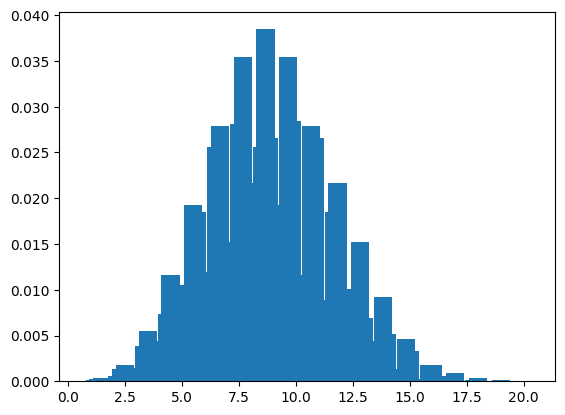
\includegraphics[width=0.7\linewidth]{screenshot001}
		\caption{}
		\label{fig:screenshot001}
	\end{figure}
	\section{}
	(a) Total Permutation n!. Sample space with replacement n{\textsuperscript{n}} {$\rightarrow$} P = {$\frac{n!}{n{\textsuperscript{n}}}$}. {\newline}
	(b) Divide both side with n{\textsuperscript{n}} {\newline}
	(c) Drawing without x{\textsubscript{i}} = {$\frac{n-1}{n}$}. So P(with replacement) = ({$\frac{n-1}{n}$}){\textsuperscript{n}} = e{\textsuperscript{-1}} if n {{$\rightarrow$}} {$\infty$}{\newline}
	{\newline}
	\section{}
	Let P(i) = probability that the candidate hired on the i{\textsuperscript{th}} trial is best.
	
	P = {$\frac{1}{n - i + 1}$} 
	{\newline}
	\section{}
	P = {$\frac{.5 * 5 * .01}{.5 * 5 * .01 + .5 * .25 * .01}$}
	\section{}
	(a) P = {$\frac{1}{2}$} * {$\frac{2}{3}$} + {$\frac{1}{2}$} * {$\frac{3}{5}$} = {$\frac{19}{30}$}
	{\newline}
	(b) P = {$\frac{1}{3}$} * {$\frac{30}{19}$}
	\section{}
	Let {\textit{B}} be associated sigma algebra with B
	{\newline}
	(a) S = (* {$\vert$} B) {$\subset$} B. Also S is a finite set so P(S) {$\geq$} 0.
	{\newline}
	(b) S = B. Every set is a subset of itself So P(B {$\vert$} B) = 1
	{\newline}
	(c) Using definneti Let A{\textsubscript{1}} and A{\textsubscript{2}} {$\in$} {\textit{B}} and they are disjoint. So P(A{\textsubscript{1}} {$\cup$} B{\textsubscript{2}} {$\vert$} ) = P(A{\textsubscript{1}} {$\vert$} B) + P(A{\textsubscript{2}} {$\vert$} B) + 0 (intersection is 0).
	{\newline}
	\section{}
	(a){$\vert$}(b) P = {$\frac{1 - P(probability for not hitting 8, 9, 10 times)}{P(probability for not hitting 9, 10 times)}$} = .9922
	\section{}
	Referring to Example 1.3.4
	{\newline}
	(a) S = P(A{$\vert$}{\textit{W}}) = {$\frac{P(A \cap {\textit{W}})}{P({\textit{W}})}$}
	P({\textit{W}}) = {Warden sen B to die} = {$\frac{\gamma}{3}$} + 1/3 + 0 = {$\frac{\gamma + 1}{3}$}
	{\newline}
	S = {$\frac{\gamma}{3}$} / {$\frac{\gamma + 1}{3}$} = {$\frac{\gamma}{\gamma + 1}$} = {$\frac{1}{3}$} {$\in$} {$\gamma$} = .5
	{\newline}
	(b) P(B {$\vert$} W) = 0, P(A {$\vert$} {\textit{W}}) = {$\frac{1}{3}$}
	So P{C {$\vert$} {\textit{W}}} = {$\frac{2}{3}$}
	So fate change is beneifical for A.
	{\newline}
	\section{}
	(a) P(B) = 1; So B = U where U is universal set. P(A{$\vert$}B) = P(A)
	{\newline}
	(b) A {$\subset$} B {$\Rightarrow$} P(A {$\cap$} B) = P(A); P(B{$\vert$}A) = {$\frac{P(A \cap B)}{P(A)}$} = {$\frac{P(A)}{P(A)}$} = 1 {$\Rightarrow$} P(A{$\vert$}B) = {$\frac{P(A)}{P(B)}$}
	{\newline}
	(c) P(A {$\vert$} (A $\cup$ B)) = {$\frac{P(A \cap (A \cup B))}{P(A \cup B)}$} = {$\frac{P(A)}{P(A) + P(B)}$}
	{\newline}
	(d) P(A {$\cap$} B {$\cap$} C) = {$\frac{P(A \cap B \cap C)}{P(B \cap C)}$} * {$\frac{P(B \cap C)}{P(C)}$} * P(C) {$\Rightarrow$} P(A {$\vert$} (B {$\cap$} B))P(B{$\vert$}C)(P(C))
	{\newline}
	
	\section{}
	(a)(b) P(A {$\cap$} B) = P(A) * P(B) Independent Event
	P(A {$\cap$} B) = 0 (Mutually Exclusive Event). Hence both cant occur together.
	
	\section{}
	(b) P(B {$\cap$} A{\textsuperscript{C}}) = P(B) - P(B {$\cap$} A) {$\Rightarrow$} P(B)(1 - P(A)) = P(B)P(A{\textsuperscript{C}})
	{\newline}
	(c) P(A{\textsuperscript{C}} {$\cap$} B{\textsuperscript{C}}) = P(U(universal set)) - P(A {$\cup$} B) = 1 - (P(A) + P(B) - P(A {$\cap$} B)) = 1 - (1 - P(A{\textsuperscript{c}}) + 1 - P(B{\textsuperscript{c}}) + (1 - P(A{\textsuperscript{c}})(1 - P(B{\textsuperscript{c}}))) = P(A{\textsuperscript{C}}) * P(B{\textsuperscript{C}})
	
	\section{}
	(a) P(dash) = {$\frac{2}{3}$} * {$\frac{4}{7}$} + {$\frac{1}{4}$} * {$\frac{3}{7}$} = {$\frac{41}{84}$} P(conditional) = {$\frac{32}{41}$}
	{\newline}
	(b) By similar calculation P(dot-dot | dot-dot) = .4132, P(dot-dash | dot-dot) = .2448, P(dash-dot | dot-dot) = .14512, P(dash-dash | dot-dot) = .24488
	{\newline}
	\section{}
	% TODO: \usepackage{graphicx} required
	\begin{figure}
		\centering
		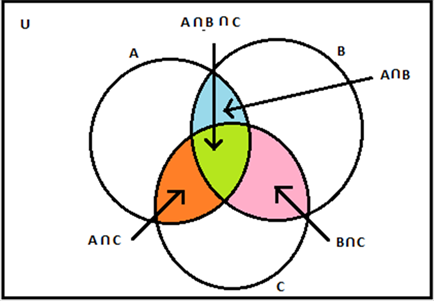
\includegraphics[width=0.7\linewidth]{screenshot002}
		\caption{}
		\label{fig:screenshot002}
	\end{figure}
	(a)(Figure 1.2) Lets consider it through A, B, C So E{\textsuperscript{1}} = Set of Points in A, B, C only (None in there intersection)
	E{\textsuperscript{2}} are all points in the intersection pairwise but not in all three we need to exclude it. E{\textsuperscript{3}} are the points in the intersection of all 3. So P(E{\textsuperscript{1}}) + P(E{\textsuperscript{2}}) + P(E{\textsuperscript{3}}) = P(A {$\cup$} B {$\cup$} C) The concept be extended to k, n generic form
	{\newline}
	(b) Now apply Exclusion inclusion principle. E{\textsubscript{1}} = P(A{\textsubscript{1}} {$\cap$} A{\textsubscript{2}} {$\cap$} A{\textsubscript{3}} ... ) So For k=n, 1 term will appear. For k=n-1, that term will appear {\textsuperscript{n}C\textsubscript{n-1}} (was was neglected), for k = n-2 that term will appear {\textsuperscript{n}C\textsubscript{n-2}} ... (Its like term selection and not rearrangement). So we get the series.
	{\newline}
	(c) If A{\textsubscript{1}} $\cup$ A{\textsubscript{2}} {$\cup$} A{\textsubscript{3}} ... {$\rightarrow$} U (Universal Set) So P(U) {$\rightarrow$} 1, So the series of inclusion - exclusion principle reaches 1.
	{\newline}
	(d) This formulae is P (A {$\cup$} B {$\cup$} C) = P(A) + P(B) + P(C) - P(A {$\cap$} B) - P(A {$\cap$} C) - P(B {$\cap$} C) + P(A {$\cap$} B {$\cap$} C) 
	{\newline}
	\section{}
	(a) (Bonferroni's Inequality) P(A {$\cup$} B) = P(A) + P(B) - P(A {$\cap$} B). P(U) where U is universal set {$\Rightarrow$} P(U) = 1; 1 > P(A) + P(B) - P(A {$\cap$} B) {$\Rightarrow$} P(A {$\cap$} B) > P(A) + P(B) - 1
	
	(Boole's Inequality) 
	P($\bigcup\limits_{i=1}^{\infty} P_{i}$) < {$\sum$ P\textsubscript{i}}, Which is logical because the union consider only one element, but in summation sample points are repeated in some or the other way.
	{\newline}
	(b) Let P{\textsubscript{i}} = P(A{\textsubscript{1}} {$\cap$} A{\textsubscript{2}} {$\cap$} ... A{\textsubscript{i}}). Any further intersection would lead to reduction of elements. Hence P(\textsubscript{i}) > P(\textsubscript{j}) on j > i
	{\newline}
	(c) P({$\bigcup$} A) = 1, Rest of terms will follow the sequence k - {\textsuperscript{k}}C{\textsubscript{1}} + {\textsuperscript{k}}C{\textsubscript{2}} - ... {$\pm$} {\textsuperscript{k}}C{\textsubscript{k}}
	
	\section{}
	{$\sum_{i=10}^{20}$} {\textsuperscript{20}}C{\textsubscript{i}}{($\frac{1}{4})$}{\textsuperscript{k}}{($\frac{3}{4}$)}{\textsuperscript{20-k}}
	
	\section{}
	P{\textsubscript{X}}(X = x{\textsubscript{i}}) = P({s{\textsubscript{j} {$\in$} S : X(s{\textsubscript{j}) = x{\textsubscript{j}}}}})
	{$\mathcal{X}$} = [ x{\textsubscript{1}, x\textsubscript{2}, x{\textsubscript{3} ... x{\textsubscript{m}}}} ]
	{\newline}
	(a) Its defined in a probability sapce so P{\textsubscript{X}} {$\ge$} 0
	{\newline}
	(b) Let x{\textsubscript{k}} = S So P{\textsubscript{X}}(x{\textsubscript{k}}) = 1 Hence 2
	{\newline}
	(c) x{\textsuperscript{j}} is a real space so its already have a sigma algebra, also all of its subset are in sigma algebra. Hence is a std problem.
	{\newline}
	
	\section{}
	calculation
	
	\section{}
	(a) {$\lim_{x {\rightarrow} -{\infty}}$}({$\frac{1}{2}$} + {$\frac{1}{\pi}$} * tan{\textsuperscript{-1}}(x), x {$\in$} (-{$\infty$}, {$\infty$})) = 0 and {$\lim_{x {\rightarrow} {\infty}}$}({$\frac{1}{2}$} + {$\frac{1}{\pi}$} * tan{\textsuperscript{-1}}(x), x {$\in$} (-{$\infty$}, {$\infty$})) = 1 
	{$\frac{dF}{dx}$} {$\sim$} {$\frac{1}{1 + x{\textsuperscript{2}}}$} > 0
	So F{\textsuperscript{'}}(x) > 0 at all x, hence right continuous.
	
	(b), (c), (d) are same
	
	\section{}
	Let F(x) be a cdf. So by definition F(x) = P{\textsubscript{X}}(X {$\le$} x), for all x {$\in$} X. P{\textsubscript{X}}(X = x{\textsubscript{i}}) = P({s{\textsubscript{j}} {$\in$} S : X(s{\textsubscript{j}}) = x{\textsubscript{i}}})
	{\newline}
	(a) {$\lim_{x {\rightarrow} -{\infty}}F(x) = 0$} {$\Rightarrow$} {$\lim_{x {\rightarrow} -{\infty}}P{\textsubscript{X}}(X {\le} x)$} {$\Rightarrow$} P{\textsubscript{X}}(s{\textsubscript{j} {$\in$} S : X(s{\textsubscript{j}) {$\le$} x{\textsubscript{j}})} when x{\textsubscript{j}} {$\rightarrow$} -{$\infty$}, count of s{\textsubscript{j}}'s {$\rightarrow$} 0 Hence P{\textsubscript{X}} {$\rightarrow$} 0
		
	{$\lim_{x {\rightarrow} {\infty}}F(x) = 1$} => {$\lim_{x {\rightarrow} {\infty}}$} P{\textsubscript{X}(X {$\le$} x)} {$\Rightarrow$} P{\textsubscript{X}}(s{\textsubscript{j}} {$\in$} S : X(s{\textsubscript{j} {$\le$} x{\textsubscript{j}}})). As x{\textsubscript{j}} {$\rightarrow$} {$\infty$} count of s{\textsuperscript{j}}'s {$\rightarrow$} N where N is number of subset of S or all sample points. Hence P{\textsubscript{X}}} {$\rightarrow$} 1
	{\newline}
	(b) Let x{\textsubscript{i}} > x{\textsubscript{j}} {$\Rightarrow$} P{\textsubscript{Xi}} will have more than or equal to elements of S then P{\textsubscript{Xi}} (By definition) {$\Rightarrow$} P{\textsubscript{Xi}} {$\ge$} P{\textsubscript{Xy}}. Hence its a non decreasing function.
	{\newline}
	(c) Let count(s{\textsuperscript{i}}) = a for X {$\le$} x{\textsubscript{i}}, Since (b) Let count(s{\textsuperscript{j}}) = a+1 for X {$\le$} x{\textsubscript{j}}, So at x{\textsubscript{j}} the F will have a value different than a point just behind x{\textsubscript{j}} will have value of P{\textsubscript{X}}{x{\textsubscript{i}}} Hence its a right continuous
	{\newline}
	
	\section{}
	F{\textsubscript{X}} {$\ge$} F{\textsubscript{Y}}. X {$\sim$} F{\textsubscript{X}}(t) and Y {$\sim$} F{\textsubscript{X}}(t) {$\rightarrow$} P{\textsubscript{X}}(X {$\ge$} x) {$\ge$} P{\textsubscript{Y}}(Y {$\le$} y) 
	
	-P{\textsubscript{X}}(X {$\le$} x) {$\ge$} -P{\textsubscript{Y}}(Y {$\le$} y) 
	
	1 - P(X {$\le$} t) {$\ge$} 1 - P(X {$\le$} t) for every t
	
	
	P(X > t) {$\ge$} P(X > t) for every t
	
	\section{}
	{$\sum_{k=1}^{n}$} t{\textsuperscript{k-1}} = {$\frac{1 - t{\textsuperscript{n}}}{1 - t}$}
	
	{$\sum_{k=1}^{n}$} t{\textsuperscript{k-1}} + t{\textsuperscript{n}} = {$\frac{1 - t{\textsuperscript{n}}}{1 - t}$} + t{\textsuperscript{n}} = {$\frac{1 - t{\textsuperscript{n+1}}}{1 - t}$}
	{\newline}
	
	{$\sum_{k=1}^{n+1}$} t{\textsuperscript{k-1}} = {$\frac{1 - t{\textsuperscript{n+1}}}{1 - t}$}
	
	\section{}
	pmf(X = 0) = {$\frac{({\textsuperscript{25}C{\textsubscript{4}}})}{{\textsuperscript{30}C{\textsubscript{4}}}}$}
	{\newline}
	pmf(X = 1) = {$\frac{({\textsuperscript{25}C{\textsubscript{3}}}) * ({\textsuperscript{5}C{\textsubscript{3}}})}{{\textsuperscript{30}C{\textsubscript{4}}}}$}
	{\newline}
	pmf(X = 2) = {$\frac{({\textsuperscript{25}C{\textsubscript{2}}}) * ({\textsuperscript{5}C{\textsubscript{2}}})}{{\textsuperscript{30}C{\textsubscript{4}}}}$}
	{\newline}
	pmf(X = 3) = {$\frac{({\textsuperscript{25}C{\textsubscript{1}}}) * ({\textsuperscript{5}C{\textsubscript{1}}})}{{\textsuperscript{30}C{\textsubscript{4}}}}$}
	{\newline}
	pmf(X = 4) = {$\frac{({\textsuperscript{25}C{\textsubscript{0}}}) * ({\textsuperscript{5}C{\textsubscript{0}}})}{{\textsuperscript{30}C{\textsubscript{4}}}}$}
	{\newline}
	
	\section{}
	{$\int_{-{\infty}}^{{\infty}}$}g(x) = {$\int_{-{\infty}}^{x{\textsubscript{0}}}$} * 0 + {$\int_{x{\textsubscript{0}}}^{{\infty}}$}{$\frac{f(x)}{[1 - F(x{\textsubscript{0}})]}$} = {$\frac{1 - F(x{\textsubscript{0}})}{1 - F(x{\textsubscript{0}})}$} = 1 g(x) {$\ge$} 0 Hence proved
	
	\section{}
	(a) {$\lim_{y {\rightarrow} 1}$} = 1 - {$\frac{1}{y1{\textsuperscript{2}}}$} = 0
	{\newline}
	{$\lim_{y {\rightarrow} {\infty}}$} = 1 - {$\frac{1}{{\infty}{\textsuperscript{2}}}$} = 1
	{\newline}
	by differentiating it can be proven F{\textsubscript{Y}} is non decreasing
	{\newline}
	F{\textsubscript{Y}} is right continuous
	{\newline}
	(b) pdf(y) = {$\frac{2}{y_{3}}$}
	{\newline}
	(c) nonsense question
	
	\section{}
	(a) c = 1
	{\newline}
	(b) c = {$\frac{1}{2}$}
	
	\section{}
	skipping by same logic!
	
	
	
	
	
	
	
	
	
	
	
	
\end{document}